\documentclass[english,floatsintext,man]{apa6}

\usepackage{amssymb,amsmath}
\usepackage{ifxetex,ifluatex}
\usepackage{fixltx2e} % provides \textsubscript
\ifnum 0\ifxetex 1\fi\ifluatex 1\fi=0 % if pdftex
  \usepackage[T1]{fontenc}
  \usepackage[utf8]{inputenc}
\else % if luatex or xelatex
  \ifxetex
    \usepackage{mathspec}
    \usepackage{xltxtra,xunicode}
  \else
    \usepackage{fontspec}
  \fi
  \defaultfontfeatures{Mapping=tex-text,Scale=MatchLowercase}
  \newcommand{\euro}{€}
\fi
% use upquote if available, for straight quotes in verbatim environments
\IfFileExists{upquote.sty}{\usepackage{upquote}}{}
% use microtype if available
\IfFileExists{microtype.sty}{\usepackage{microtype}}{}

% Table formatting
\usepackage{longtable, booktabs}
\usepackage{lscape}
% \usepackage[counterclockwise]{rotating}   % Landscape page setup for large tables
\usepackage{multirow}		% Table styling
\usepackage{tabularx}		% Control Column width
\usepackage[flushleft]{threeparttable}	% Allows for three part tables with a specified notes section
\usepackage{threeparttablex}            % Lets threeparttable work with longtable

% Create new environments so endfloat can handle them
% \newenvironment{ltable}
%   {\begin{landscape}\begin{center}\begin{threeparttable}}
%   {\end{threeparttable}\end{center}\end{landscape}}

\newenvironment{lltable}
  {\begin{landscape}\begin{center}\begin{ThreePartTable}}
  {\end{ThreePartTable}\end{center}\end{landscape}}




% The following enables adjusting longtable caption width to table width
% Solution found at http://golatex.de/longtable-mit-caption-so-breit-wie-die-tabelle-t15767.html
\makeatletter
\newcommand\LastLTentrywidth{1em}
\newlength\longtablewidth
\setlength{\longtablewidth}{1in}
\newcommand\getlongtablewidth{%
 \begingroup
  \ifcsname LT@\roman{LT@tables}\endcsname
  \global\longtablewidth=0pt
  \renewcommand\LT@entry[2]{\global\advance\longtablewidth by ##2\relax\gdef\LastLTentrywidth{##2}}%
  \@nameuse{LT@\roman{LT@tables}}%
  \fi
\endgroup}


  \usepackage{graphicx}
  \makeatletter
  \def\maxwidth{\ifdim\Gin@nat@width>\linewidth\linewidth\else\Gin@nat@width\fi}
  \def\maxheight{\ifdim\Gin@nat@height>\textheight\textheight\else\Gin@nat@height\fi}
  \makeatother
  % Scale images if necessary, so that they will not overflow the page
  % margins by default, and it is still possible to overwrite the defaults
  % using explicit options in \includegraphics[width, height, ...]{}
  \setkeys{Gin}{width=\maxwidth,height=\maxheight,keepaspectratio}
\ifxetex
  \usepackage[setpagesize=false, % page size defined by xetex
              unicode=false, % unicode breaks when used with xetex
              xetex]{hyperref}
\else
  \usepackage[unicode=true]{hyperref}
\fi
\hypersetup{breaklinks=true,
            pdfauthor={},
            pdftitle={The emergence of words from vocal imitations},
            colorlinks=true,
            citecolor=blue,
            urlcolor=blue,
            linkcolor=black,
            pdfborder={0 0 0}}
\urlstyle{same}  % don't use monospace font for urls

\setlength{\parindent}{0pt}
%\setlength{\parskip}{0pt plus 0pt minus 0pt}

\setlength{\emergencystretch}{3em}  % prevent overfull lines

\ifxetex
  \usepackage{polyglossia}
  \setmainlanguage{}
\else
  \usepackage[english]{babel}
\fi

% Manuscript styling
\captionsetup{font=singlespacing,justification=justified}
\usepackage{csquotes}
\usepackage{upgreek}

 % Line numbering
  \usepackage{lineno}
  \linenumbers


\usepackage{tikz} % Variable definition to generate author note

% fix for \tightlist problem in pandoc 1.14
\providecommand{\tightlist}{%
  \setlength{\itemsep}{0pt}\setlength{\parskip}{0pt}}

% Essential manuscript parts
  \title{The emergence of words from vocal imitations}

  \shorttitle{Words from imitations}


  \author{Pierce Edmiston\textsuperscript{1}, Marcus Perlman\textsuperscript{2}, \& Gary Lupyan\textsuperscript{1}}

  \def\affdep{{"", "", ""}}%
  \def\affcity{{"", "", ""}}%

  \affiliation{
    \vspace{0.5cm}
          \textsuperscript{1} University of Wisconsin-Madison\\
          \textsuperscript{2} Max Planck Institute for Psycholinguistics  }

  \authornote{
    \newcounter{author}
    Pierce Edmiston and Gary Lupyan, Department of Psychology, University of
    Wisconsin-Madison, Madison, Wisconsin. Marcus Perlman, Max Planck
    Institute for Psycholinguistics, Nijmegen, Netherlands.

                      Correspondence concerning this article should be addressed to Pierce Edmiston, 1202 W. Johnson St., Madison, WI, 53703. E-mail: \href{mailto:pedmiston@wisc.edu}{\nolinkurl{pedmiston@wisc.edu}}
                                    }


  \abstract{People have long pondered the origins of language, especially the words
that compose them. Here, we report a series of experiments investigating
how conventional spoken words might emerge from imitations of
environmental sounds. Does the repeated imitation of an environmental
sound gradually give rise to novel word forms? In what ways do these
words resemble the original sounds that motivated them? Participants
played a version of the children's game ``Telephone''. The first
generation of participants imitated recognizable environmental sounds
(e.g., glass breaking, water splashing). Subsequent generations imitated
the imitations for a maximum of 8 generations. The results showed that
the imitations became more stable and word-like, and later imitations
were easier to learn as category labels. At the same time, even after 8
generations, both spoken imitations and their written transcriptions
could be matched above chance to the category of environmental sound
that motivated them. These results show how repeated imitation can
create progressively more word-like forms while continuing to retain a
resemblance to the original sound that motivated them, and speak to the
possible role of human vocal imitation in explaining the origins of at
least some spoken words.}
  \keywords{language evolution, iconicity, vocal imitation, transmission chain \\

    \indent Word count: 5552
  }

\usepackage[titles]{tocloft}
\cftpagenumbersoff{figure}
\renewcommand{\cftfigpresnum}{\itshape\figurename\enspace}
\renewcommand{\cftfigaftersnum}{.\space}
\setlength{\cftfigindent}{0pt}
\setlength{\cftafterloftitleskip}{0pt}
\settowidth{\cftfignumwidth}{Figure 10.\qquad}

\cftpagenumbersoff{table}
\renewcommand{\cfttabpresnum}{\itshape\tablename\enspace}
\renewcommand{\cfttabaftersnum}{.\space}
\setlength{\cfttabindent}{0pt}
\setlength{\cftafterloftitleskip}{0pt}
\settowidth{\cfttabnumwidth}{Table 10.\qquad}



\usepackage{amsthm}
\newtheorem{theorem}{Theorem}
\newtheorem{lemma}{Lemma}
\theoremstyle{definition}
\newtheorem{definition}{Definition}
\newtheorem{corollary}{Corollary}
\newtheorem{proposition}{Proposition}
\theoremstyle{definition}
\newtheorem{example}{Example}
\theoremstyle{remark}
\newtheorem*{remark}{Remark}
\begin{document}

\maketitle

\setcounter{secnumdepth}{0}



The importance of imitation and depiction in the origin of signs is
clearly observable in signed languages (Goldin-Meadow, 2016; Kendon,
2014; Klima \& Bellugi, 1980), but in considering the idea that
imitation in the vocal modality may be key to understanding the origin
of spoken words, many have argued that the human capacity for vocal
imitation is far too limited to play a significant role (Arbib, 2012;
Armstrong \& Wilcox, 2007; Corballis, 2003; Hewes, 1973; Hockett, 1978;
Tomasello, 2010). For example, Pinker and Jackendoff (2005) argued that,
\enquote{most humans lack the ability\ldots{} to convincingly reproduce
environmental sounds\ldots{} Thus \enquote{capacity for vocal imitation}
in humans might be better described as a capacity to learn to produce
speech} (p.~209). Consequently, it is still widely assumed that vocal
imitation --- or more broadly, the use of any sort of resemblance
between form and meaning --- cannot be important to understanding the
origin of spoken words. We challenge this view by demonstrating that
spoken words can emerge from vocal imitations even without the intention
to communicate. We find that repeating vocal imitations of environmental
sounds over generations of unique speakers is sufficient to create more
word-like vocalizations both in form and function.

Although most words of contemporary spoken languages are not clearly
imitative in origin, there has been a growing recognition of the
importance of imitative words in spoken languages (Dingemanse, Blasi,
Lupyan, Christiansen, \& Monaghan, 2015; Perniss, Thompson, \&
Vigliocco, 2010) and the frequent use of vocal imitation and depiction
in spoken discourse (Clark \& Gerrig, 1990; Lewis, 2009). This has led
some to argue for the importance of imitation for understanding the
origin of spoken words (e.g., Brown, Black, \& Horowitz, 1955;
Dingemanse, 2014; Donald, 2016; Imai \& Kita, 2014; Perlman, Dale, \&
Lupyan, 2015). In addition, counter to previous assumptions, people are
highly effective at using vocal imitations to refer to environmental
sounds such as coins dropping in a jar or mechanical events such as
scraping --- in some cases, even more effective than when using
conventional words (Lemaitre \& Rocchesso, 2014). Recent work has also
shown that people are able to create novel imitative vocalizations for
more abstract meanings (e.g. \enquote{slow}, \enquote{rough},
\enquote{good}, \enquote{many}) that are understandable to naïve
listeners (Perlman et al., 2015). These imitations are effective not
because people can mimic environmental sounds with high fidelity, but
because people are able to produce imitations that capture the salient
features of sounds in ways that are understandable to listeners
(Lemaitre, Houix, Voisin, Misdariis, \& Susini, 2016). Similarly, the
features of onomatopoeic words might highlight distinctive aspects of
the sounds they represent. For example, the initial voiced, plosive
\texttt{/b/} in \enquote{boom} represents an abrupt, loud onset, the
back vowel \texttt{/u/} a low pitch, and the nasalized \texttt{/m/} a
slow, muffled decay (Rhodes, 1994).

Thus, converging evidence suggests that people can use vocal imitation
as an effective means of communication. But can vocal imitations ever
give rise to words that can be integrated into the vocabulary of a
language? And if so, by what means might this happen? To answer these
questions, we recruited participants to play an online version of the
children's game of \enquote{Telephone}. In the children's game, a spoken
message is whispered from one person to the next. In our version, the
original message or \enquote{seed sound} was a recording of an
environmental sound. The initial group of participants (first
generation) imitated these seed sounds, the next generation imitated the
previous imitators, and so on for up to 8 generations.

We then conducted a series of analyses and additional experiments to
systematically answer the following questions: First, do imitations
stabilize in form and become more word-like as they are repeated?
Second, do the imitations retain a resemblance to the original
environmental sound that inspired them? If so, it should be possible for
naïve participants to match the emergent words back to the original seed
sounds. Third, do the imitations become more suitable as labels for the
category of sounds that motivated them? For example, does the imitation
of a particular water-splashing sound become, over generations of
repeated imitation, a better label for the more general category of
water-splashing sounds?

\section{Experiment 1: Stabilization of imitations through
repetition}\label{experiment-1-stabilization-of-imitations-through-repetition}

In the first experiment, we collected the vocal imitations, and assessed
the extent to which repeating imitations of environmental sounds over
generations of unique speakers results in progressive stabilization
toward more word-like forms. After collecting the imitations, we
measured changes in the stability of the imitations in three ways.
First, we measured changes in the perception of acoustic similarity
between subsequent generations of imitations along contiguous
transmission chains. Second, we used algorithmic measures of acoustic
similarity to assess the similarity of imitations sampled within and
between transmission chains. Third, we obtained transcriptions of
imitations, and measured the extent to which later generation imitations
were transcribed with greater consistency and agreement. The results
show that repeated imitation results in vocalizations that are easier to
repeat with high fidelity and easier to transcribe into English
orthography.

\subsection{Methods}\label{methods}

\subsubsection{Selecting seed sounds}\label{selecting-seed-sounds}

To avoid sounds having lexicalized or conventionalized onomatopoeic
forms in English, we used inanimate categories of environmental sounds.
Using an odd-one-out norming procedure (\emph{N}=105 participants), an
initial set of 36 sounds in 6 categories was reduced to a final set of
16 \enquote{seed} sounds: 4 sounds in each of 4 categories. The purpose
of this norming procedure was to reach a set of approximately equally
distinguishable sounds within each category by systematically removing
the sounds that stood out in each category. The results of the norming
procedure are shown in Fig. S1. The four final categories were: water,
glass, tear, zipper. The final 16 seed sounds can be downloaded from
here: \href{https://osf.io/n6g7d/download}{osf.io/n6g7d/download}.

\subsubsection{Collecting vocal
imitations}\label{collecting-vocal-imitations}

Participants (\emph{N}=94) recruited from Amazon Mechanical Turk were
paid to participate in an online version of the children's game of
\enquote{Telephone}. Participants were instructed that they would hear
some sound and their task is to reproduce it as accurately as possible
using their computer microphone. Full instructions are provided in the
Supplemental Materials.

Each participant listened to and imitated four sounds: one from each of
the four categories of environmental sounds. Sounds were assigned at
random such that participants were unlikely to imitate the same person
more than once. Participants were allowed to listen to each target sound
multiple times, but were only allowed a single recording in response.
Recordings that were too quiet (less than -30 dBFS) were not accepted.

Imitations were monitored by an experimenter to catch any gross errors
in recording before they were heard by the next generation of imitators.
For example, recordings with loud sounds in the background were removed,
and recordings were trimmed to the length of the imitation prior to the
next generation. The experimenter also removed sounds that violated the
rules of the experiment, e.g., by saying something in English. A total
of 115 (24\%) imitations were removed prior to subsequent analysis. The
final sample contained 365 imitations along 105 contiguous transmission
chains (Fig. 1).

\begin{figure}
\centering
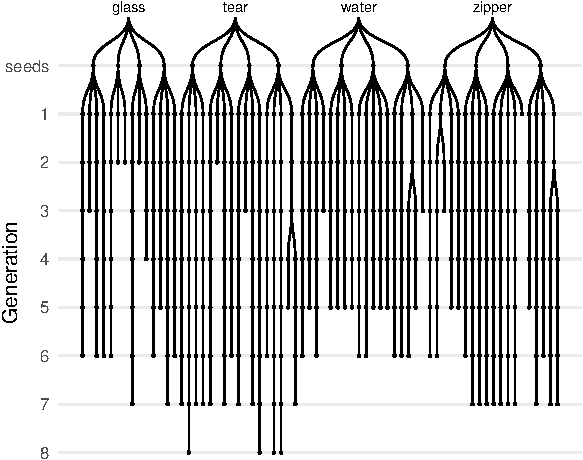
\includegraphics{fig1-1.pdf}
\caption{\label{fig:fig1}Vocal imitations collected in the transmission
chain experiment. Seed sounds (16) were sampled from four categories of
environmental sounds: glass, tear, water, zipper. Participants imitated
each seed sound, and then the next generation of participants imitated
the imitations, and so on, for up to 8 generations. Chains are
unbalanced due to random assignment and the exclusion of some low
quality recordings.}
\end{figure}

\subsubsection{Measuring acoustic
similarity}\label{measuring-acoustic-similarity}

\paragraph{Acoustic similarity
judgments}\label{acoustic-similarity-judgments}

Acoustic similarity judgments were gathered from five research
assistants who listened to pairs of sounds (approx. 300) and rated their
subjective similarity. On each trial, raters heard two sounds from
subsequent generations played in random order. They then indicated the
similarity between the sounds on a 7-point Likert scale from
\emph{Entirely different and would never be confused} to \emph{Nearly
identical}. Raters were encouraged to use as much of the scale as they
could while maximizing the likelihood that, if they did this procedure
again, they would reach the same judgments. Full instructions are
provided in the Supplemental Materials. Inter-rater reliability was
calculated as the intra-class coefficient treating the group as the unit
of analysis (Gamer, Lemon, Fellows, \& Singh, 2012; Shrout \& Fleiss,
1979): ICC = 0.76, 95\% CI {[}0.70, 0.81{]}, F(170, 680) = 4.18,
\emph{p} \textless{} 0.001. Ratings were normalized for each rater
(z-scored) prior to analysis.

\paragraph{Algorithmic acoustic
similarity}\label{algorithmic-acoustic-similarity}

To obtain algorithmic measures of acoustic similarity, we used the
acoustic distance functions included in Phonological Corpus Tools (Hall,
Allen, Fry, Mackie, \& McAuliffe, 2016). We computed Mel-frequency
cepstral coefficients (MFCCs) between pairs of imitations using 12
coefficients in order to obtain speaker-independent estimates.

\subsubsection{Collecting transcriptions of
imitations}\label{collecting-transcriptions-of-imitations}

Participants (\emph{N}=216) recruited from Amazon Mechanical Turk were
paid to transcribe vocalizations using English orthography, being
instructed to write down what they heard as a single \enquote{word} so
that the written word would sound as much like the sound as possible.
Participants were instructed that this was a word creation task and so
to avoid transcribing the vocalizations into existing English words.
Each participant completed 10 transcriptions. Transcriptions were
gathered for the first and the last three generations of imitations
collected in the transmission chain experiment. Participants also
provided \enquote{transcriptions} of the original environmental seed
sounds. Analyses of these transcriptions are reported in the
Supplementary Materials (Fig. S5).

To measure similarity among transcriptions of the same imitation, we
used the \texttt{SequenceMatcher} functions in the \texttt{difflib}
package of the Python standard library, which implements a version of
Ratcliff and Obershelp's \enquote{gestalt pattern matching} algorithm.
Alternative measures of transcription agreement including exact string
matching and the length of the longest substring match were also
collected.

\subsubsection{Analyses}\label{analyses}

Statistical analyses were conducted in R using linear mixed-effects
models provided by the \texttt{lme4} package (Bates, Mächler, Bolker, \&
Walker, 2015). Degrees of freedom and corresponding significance tests
for linear mixed-effects models were estimated using the Satterthwaite
approximation via the \texttt{lmerTest} package (Kuznetsova, Bruun
Brockhoff, \& Haubo Bojesen Christensen, 2016). Random effects
(intercepts and slopes) for subjects and for items were included
wherever appropriate, and are described below.

\subsubsection{Data availability}\label{data-availability}

Our data along with all methods, materials, and analysis scripts, are
available in public repositories described on the Open Science Framework
page for this research here: \href{https://osf.io/3navm}{osf.io/3navm}.

\subsection{Results}\label{results}

\subsubsection{Acoustic similarity increased through
iteration}\label{acoustic-similarity-increased-through-iteration}

Imitations of environmental sounds became more stable over the course of
being repeated as revealed by increasing acoustic similarity judgments
along individual transmission chains. Acoustic similarity ratings were
fit with a linear mixed-effects model predicting perceived acoustic
similarity from generation with random effects (intercepts and slopes)
for raters. To test whether the hypothesized increase in acoustic
simliarity was true across all seed sounds and categories, we added
random effects (intercepts and slopes) for seed sounds nested within
categories. The results showed that, across raters and seeds, imitations
from later generations were rated as sounding more similar to one
another than imitations from earlier generations, \emph{b} = 0.10 (SE =
0.03), \emph{t}(11.9) = 3.03, \emph{p} = 0.011 (Fig. 2). This result
suggests that imitations became more stable (i.e., easier to imitate
with high fidelity) with each generation of repetition.

\begin{figure}
\centering
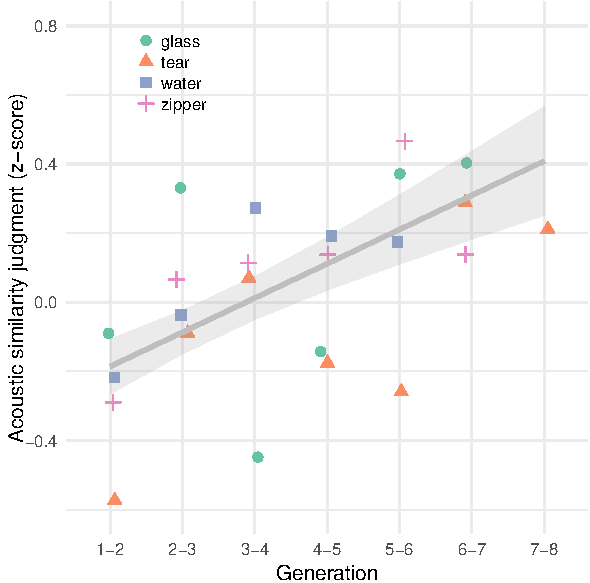
\includegraphics{fig2-1.pdf}
\caption{\label{fig:fig2}Change in perception of acoustic similarity over
generations of iterated imitation. Points depict mean acoustic
similarity ratings for pairs of imitations in each category. The
predictions of the linear mixed-effects model are shown with ±1 SE.
Acoustic similarity increased over generations, indicating that
repetition made the vocalizations easier to imitate with high fidelity.}
\end{figure}

\subsubsection{Acoustic similarity was highest within transmission
chains}\label{acoustic-similarity-was-highest-within-transmission-chains}

Increasing similarity along transmission chains could also reflect the
continuous degradation of the signal due to repeated imitation, in which
case we would expect acoustic similarity to increase both within as well
as between transmission chains as a function of generation of imitation.
To rule out this alternative explanation, we calculated MFCCs for pairs
of sounds sampled from within and between different transmission chains
from consecutive generations across categories. To analyze the results,
we fit a linear model predicting normalized acoustic similarity scores
(z-scores) from the generation of sounds. A hierarchical model was not
appropriate for this analysis because the between-chain pairs of sounds
were sampled from different categories, preventing any random effects
due to category or seed from being included in the model. We found that
acoustic similarity increased within chains more than it increased
between chains, \emph{b} = -0.07 (SE = 0.03), \emph{t}(6674.0) = -2.13,
\emph{p} = 0.033 (Fig. S2). This result supports the conclusion that
transmission chains were stabilizing on divergent acoustic forms as
opposed to all chains converging on similar forms through continuous
degradation.

\subsubsection{Later generation imitations were transcribed more
consistently}\label{later-generation-imitations-were-transcribed-more-consistently}

An additional test of stabilization and word-likeness was to measure
whether later generation imitations were transcribed more consistently
than first generation imitations. We collected a total of 2163
transcriptions --- approximately 20 transcriptions per sound. Of these,
179 transcriptions (8\%) were removed because they contained English
words. Some examples of the final transcriptions are presented in Table
1.

\begin{table}

\caption{\label{tab:table1}Examples of words transcribed from imitations.}
\centering
\begin{tabular}[t]{l|r|l|l}
\hline
Category & Seed & First generation & Last generation\\
\hline
glass & 1 & tingtingting & deetdedededeet\\
\hline
glass & 2 & chirck & correcto\\
\hline
glass & 3 & dirrng & wayew\\
\hline
glass & 4 & boonk & baroke\\
\hline
tear & 1 & scheeept & cheecheea\\
\hline
tear & 2 & feeshefee & cheeoooo\\
\hline
tear & 3 & hhhweerrr & chhhhhhewwwe\\
\hline
tear & 4 & ccccchhhhyeaahh & shhhhh\\
\hline
water & 1 & boococucuwich & eeverlusha\\
\hline
water & 2 & chwoochwooochwooo & cheiopshpshcheiopsh\\
\hline
water & 3 & atoadelchoo & mowah\\
\hline
water & 4 & awakawush & galonggalong\\
\hline
zipper & 1 & euah & izoo\\
\hline
zipper & 2 & zoop & veeeep\\
\hline
zipper & 3 & arrgt & owww\\
\hline
zipper & 4 & bzzzzup & izzip\\
\hline
\end{tabular}
\end{table}

To measure the similarity among transcriptions, we calculated the
orthographic distance between the most frequent transcription and all
other transcriptions of a given imitation. The orthographic distance
measure was a ratio based on longest contiguous matching subsequences
between pairs of transcriptions. We then fit a hierarchical linear model
predicting orthographic distance from the generation of the imitation
(First generation, Last generation) with random effects (intercepts and
slopes) for seed sound nested within category\footnote{Random effects
  for subject were not appropriate because the distance measure was
  derived from pairwise comparisons of transcriptions generated by
  different transcribers. As a result, the degrees of freedom for the
  significance tests for the parameters of this model reflect the
  Satterthwaite approximation based on the number of seed sounds (16)
  nested within categories (4), not the number of unique transcribers
  (\emph{N}=216).}. The results showed that transcriptions of last
generation imitations were more similar to one another than
transcriptions of first generation imitations, \emph{b} = -0.12 (SE =
0.03), \emph{t}(3.0) = -3.62, \emph{p} = 0.035 (Fig. 3). The same result
is reached through alternative measures of orthographic distance, such
as the percentage of exact transcription matches for each imitation,
\emph{b} = 0.10 (SE = 0.03), \emph{t}(90.0) = 2.84, \emph{p} = 0.006,
and the length of the longest matching substring, \emph{b} = 0.98 (SE =
0.24), \emph{t}(15.1) = 4.14, \emph{p} \textless{} 0.001 (Fig. S3).
Differences between transcriptions of human vocalizations and
transcriptions directly of environmental sounds are presented in the
Supplementary Materials (Fig. S5).

\begin{figure}
\centering
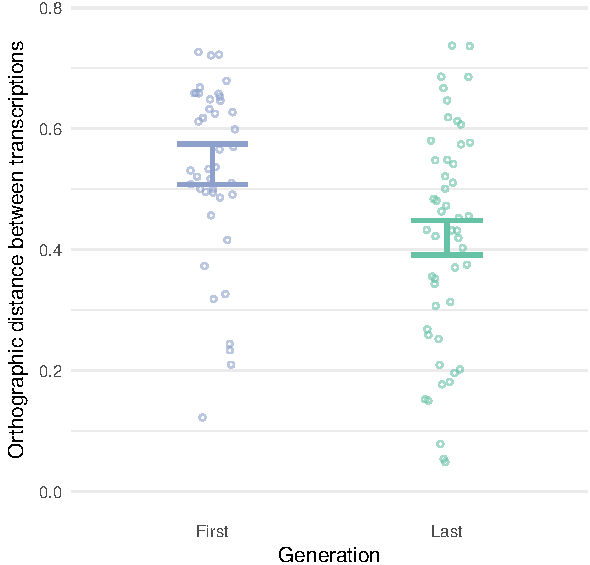
\includegraphics{fig3-1.pdf}
\caption{\label{fig:fig3}Orthographic agreement among transcriptions of
first and last generation imitations. Points depict the mean
orthographic distance between the most frequent transcription and all
other transcriptions of a given imitation, with error bars denoting ±1
SE of the hierarchical linear model predictions. Transcriptions of later
generation imitations were more similar to one another than
transcriptions of first generation imitations, suggesting that repeating
imitations made them easier to transcribe into English orthography than
direct imitations of environmental sounds.}
\end{figure}

\subsection{Discussion}\label{discussion}

Repeating imitations of environmental sounds over generations of unique
speakers was sufficient to create more wordlike forms even without any
instruction to do so. We defined wordlike-ness in terms of acoustic
stability and orthographic agreement. With additional repetitions, the
acoustic forms of the imitations became more similar to one another,
indicating they became easier to repeat with high fidelity. The
possibility that this similarity was due to uniform degradation across
all transmission chains was ruled out by algorithmic analyses of
acoustic similarity within and between chains demonstrating that
acoustic similarity increased within chains but not between them.
Additionally, later generation imitations were transcribed more
consistently into English orthography, further supporting our hypothesis
that repeating imitations makes them more word-like.

The results of Experiment 1 demonstrate the ease with which iterated
imitation gives rise to unique word forms. However, the results do not
address how these emergent words relate to the original sounds that were
being imitated. As the imitations became more word-like, were they
stabilizing on arbitrary acoustic and orthographic forms, or did they
maintain some resemblance to the environmental sounds that motivated
them? The purpose of Experiment 2 was to assess the extent to which
repeated imitations and their transcriptions maintained a resemblance to
the original set of seed sounds.

\section{Experiment 2: Resemblance of imitations to original seed
sounds}\label{experiment-2-resemblance-of-imitations-to-original-seed-sounds}

To assess the resemblance of repeated imitations to the original seed
sounds, we measured the ability of participants naïve to the design of
the experiment to match imitations and their transcriptions back to
their original sound source relative to other seed sounds from either
the same category or from different categories (Fig. 4). We used match
accuracies to answer two questions concerning the effect of iterated
imitation on resemblance to the original seed sounds. First, we asked
whether and for how many generations the imitations and their
transcriptions could be matched back to the original sounds. Second, we
asked whether repeated imitation resulted in a uniform degradation of
the signal in each imitation, or if repeated imitation resulted in some
kinds of information degrading more rapidly than others. Specifically,
we tested the hypothesis that if imitations were becoming more
word-like, then they should also be interpreted more categorically, and
thus we predicted that the imitations might lose individuating
information that identifies the specific source of an imitation more
rapidly than category information that identifies the general category
of environmental sound being imitated.

\begin{figure}
\centering
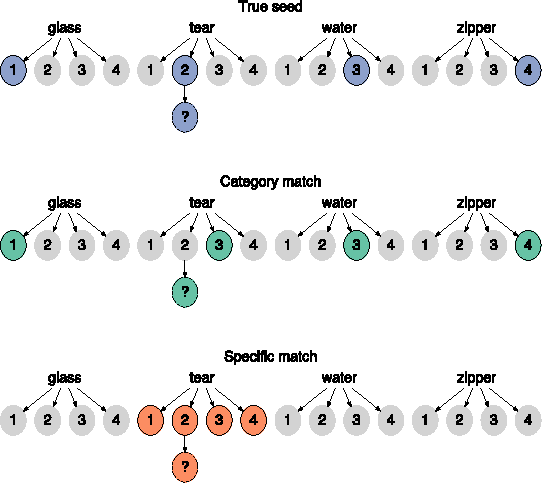
\includegraphics{fig4-1.pdf}
\caption{\label{fig:fig4}Three types of matching questions used to assess
the resemblance between the imitation (and transcriptions of imitations)
and the original seed sounds. For each question, participants listened
an imitation (dashed circles) or read a transcription of one, and had to
guess which of 4 sound choices (solid circles) they thought the person
was trying to indicate. True seed questions contained the specific sound
that generated the imitation as one of the choices (the correct
response). The remaining sound choices were sampled from different
categories. Category match questions replaced the original seed sound
with another sound from the same category. Specific match questions
pitted the actual seed against the other seeds within the same
category.}
\end{figure}

\subsection{Methods}\label{methods-1}

\subsubsection{Matching imitations to seed
sounds}\label{matching-imitations-to-seed-sounds}

Participants (\emph{N}=751) recruited from Amazon Mechanical Turk were
paid to listen to imitations, one at a time, and for each one, choose
one of four possible sounds they thought the person was trying to
imitate. The task was unspeeded and no feedback was provided.
Participants completed 10 questions at a time.

All 365 imitations were tested in each of the three question types
depicted in Fig. 4. These questions differed in the relationship between
the imitation and the four seed sounds provided as the choices in the
question. Question types (True seed, Category match, Specific match)
were assigned between-subject. Participants in the True seed and
Category match conditions were provided four seed sounds from different
categories as choices in each question. Participants in the Specific
match condition were provided four seed sounds from the same category.

\subsubsection{Matching transcriptions to seed
sounds}\label{matching-transcriptions-to-seed-sounds}

Participants (\emph{N}=468) recruited from Amazon Mechanical Turk
completed a modified version of the matching survey described above.
Instead of listening to imitations, participants now read a word (a
transcription of an imitation), which they were told was an invented
word. They were instructed that the word was invented to describe one of
the four presented sounds, and they had to guess which one. The
distractors for all questions were between-category, i.e.~true seed and
category match. Specific match questions were omitted.

Of the unique transcriptions that were generated for each sound
(imitations and seed sounds), only the top four most frequent
transcriptions were used in the matching experiment. Participants who
failed a catch trial (\emph{N}=6) were excluded, leaving 461
participants in the final sample.

\subsection{Results}\label{results-1}

\subsubsection{Imitations retained category information more than
individuating
information}\label{imitations-retained-category-information-more-than-individuating-information}

Response accuracies in matching imitations to seed sounds were fit by a
generalized linear mixed-effects model predicting match accuracy as
different from chance (25\%) based on the type of question being
answered (True seed, Category match, Specific match) and the generation
of the imitation. Question types were contrast coded using Category
match questions as the baseline condition in comparison to the other two
question types each containing the actual seed that generated the
imitation as one of the choices. The model included random intercepts
for participant\footnote{Random slopes for generation were not
  appropriate in the by-subject random effects because data collection
  was batched by generation of imitation, and therefore each participant
  did not sample across the range of generations.}, and random slopes
and intercepts for seed sounds nested within categories.

Accuracy in matching imitations to seed sounds was above chance for all
question types for the first generation of imitations, \emph{b} = 1.65
(SE = 0.14) log-odds, odds = 0.50, \emph{z} = 11.58, \emph{p}
\textless{} 0.001, and decreased steadily over generations, \emph{b} =
-0.16 (SE = 0.04) log-odds, \emph{z} = -3.72, \emph{p} \textless{}
0.001. We then tested whether this increase in difficulty was constant
across the three types of questions or if some question types became
more difficult than others. The results are shown in Fig. 5A.
Performance decreased over generations more rapidly for questions
requiring a within-category distinction than for between-category
questions, \emph{b} = -0.08 (SE = 0.03) log-odds, \emph{z} = -2.68,
\emph{p} = 0.007, suggesting that between-category information was more
resistant to loss through repeated imitation.

An alternative explanation for this result is that the within-category
match questions are simply more difficult because the sounds provided as
choices are more acoustically similar to one another than the
between-category questions, and therefore, performance might be expected
to drop off more rapidly with repeated imitation for these more
difficult questions\footnote{We observed that performance on some
  Specific match questions dropped below chance for later generations
  indicating participants had an apparent aversion to the nominally
  correct answer. Additional analyses showed that participants were not
  converging on a single incorrect response. The reason for this pattern
  is at present unclear. Removing these trials from the analysis does
  not substantively change the conclusions.}. However, performance also
decreased for the easiest type of question where the correct answer was
the actual seed generating the imitation (True seed questions; see Fig.
4); the advantage of having the true seed among between-category
distractors decreased over generations, \emph{b} = -0.07 (SE = 0.02)
log-odds, \emph{z} = -2.77, \emph{p} = 0.006. The observed increase in
the \enquote{category advantage} (i.e., the advantage of having
between-category distractors) combined with a decrease in the
\enquote{true seed advantage} (the advantage of having the actual seed
among the choices), shows that the changes induced by repeated imitation
caused the imitations to lose some of properties that linked the earlier
imitations to the specific sound that motivated them, while nevertheless
preserving a more abstract category-based resemblance.

\subsubsection{Transcriptions retained information about seed
sources}\label{transcriptions-retained-information-about-seed-sources}

We next report the results of matching the written transcriptions of the
auditory sounds back to the original environmental sounds. Remarkably,
participants were able to guess the correct meaning of a word that was
transcribed from an imitation that had been repeated up to 8 times,
\emph{b} = 0.83 (SE = 0.13) log-odds, odds = -0.18, \emph{z} = 6.46,
\emph{p} \textless{} 0.001 (Fig. 5B). This was true for True seed
questions containing the actual seed generating the transcribed
imitation, \emph{b} = 0.75 (SE = 0.15) log-odds, \emph{z} = 4.87,
\emph{p} \textless{} 0.001, and for Category match questions where
participants had to associate transcriptions with a particular category
of environmental sounds, \emph{b} = 1.02 (SE = 0.16) log-odds, \emph{z}
= 6.39, \emph{p} \textless{} 0.001. The effect of generation did not
vary across these question types, \emph{b} = 0.05 (SE = 0.10) log-odds,
\emph{z} = 0.47, \emph{p} = 0.638. The results of matching
\enquote{transcriptions} directly of the environmental sounds are shown
in Fig. S5.

\begin{figure}
\centering
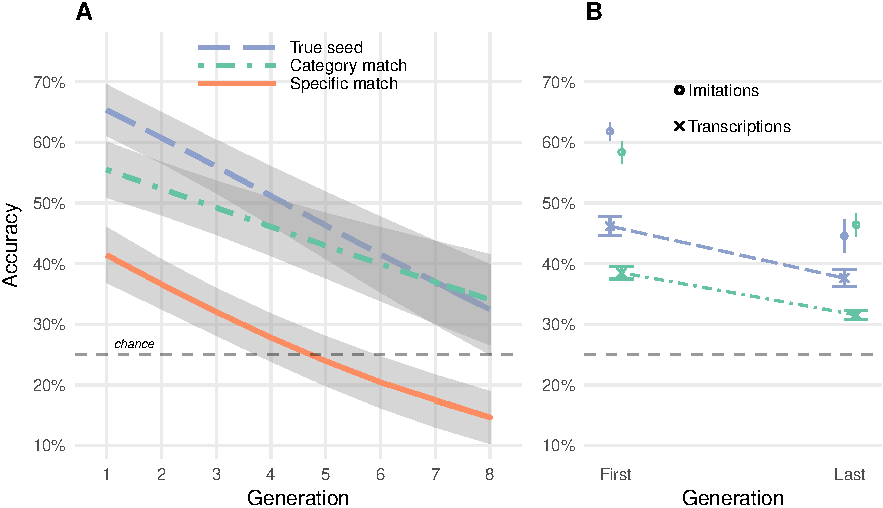
\includegraphics{fig5-1.pdf}
\caption{\label{fig:fig5}Repeated imitations retained category resemblance.
A. Accuracy of matching vocal imitations to original seed sounds as a
function of the generation during which the imitation was produced.
Curves show predictions of the generalized linear mixed effects models
with ±1 SE of the model predictions. The \enquote{category advantage}
(Category match vs.~Specific match) increased over generations, while
the \enquote{true seed advantage} (True seed v. Category match)
decreased (see main text), suggesting that imitations lose
within-category information more rapidly than between-category
information. B. Accuracy of matching transcriptions of the imitations to
original seed sounds (e.g., \enquote{boococucuwich} to a water splashing
sound). Transcriptions of imitations could still be matched back to the
category of sound that motivated the original imitation even after 8
generations. Circles show mean matching accuracy for the corresponding
vocal imitations for comparison.}
\end{figure}

\subsection{Discussion}\label{discussion-1}

Even after being repeated up to 8 times, imitations retained a
resemblance to the environmental sound that motivated them, even after
being transcribed into orthographic forms. For imitations, but not for
transcriptions, this resemblance was stronger for the category of
environmental sound than the actual seed sound, suggesting that through
repetition, the imitations were becoming more categorical. This result
supports the results of Experiment 1 in demonstrating another aspect of
wordlike-ness achieved through repeated imitation: Words, in addition to
being stable in acoustic and orthographic forms, are also categorical,
denoting all members of a category equally as opposed to identifying
individual category members. Repeating imitations of environmental
sounds is sufficient to remove some of the individuating characteristics
of the imitation while retaining a category-based resemblance.

The reason the same effect was not observed in matching accuracy for
transcriptions is unknown. One possible reason is that the process of
transcribing a non-linguistic vocalization into a written word
encourages transcribers to emphasize individuating information about the
vocalization. However, the fact that transcriptions of imitations can be
matched back to other category members (Category match questions)
suggests that transcriptions are still carrying some category
information. Another possible reason is that by subsetting the most
frequent transcriptions, we unintentionally excluded less frequent
transcriptions that were more diagnostic of category information.

Experiments 1 and 2 document a process of gradual change from an
imitation of an environmental sound to a more wordlike form. But do
these emergent words function like other words in the language? In
Experiment 3, we test the suitability of words taken from the beginning
and end of transmission chains in serving as category labels in a
category learning task.

\section{Experiment 3: Suitability of created words as category
labels}\label{experiment-3-suitability-of-created-words-as-category-labels}

One consequence of imitations becoming more word-like is that they may
make for better category labels. For example, an imitation from a later
generation, by virtue of having a more word-like form, may be easier to
learn as a label for the category of sounds that motivated it than an
earlier imitation, which is more closely yoked to a particular
environmental sound. To the extent that repeating imitations abstracts
away the idiosyncrasies of a particular category member (Edmiston \&
Lupyan, 2015; Lupyan \& Thompson-Schill, 2012), it may also be easier to
generalize to new category members. We tested these predictions using a
category learning task in which participants learned novel labels as
category labels of the seed environmental sounds. The novel labels were
transcriptions of either first or last generation imitations gathered in
Experiment 1.

\subsection{Methods}\label{methods-2}

\subsubsection{Selecting words to learn as category
labels}\label{selecting-words-to-learn-as-category-labels}

Our transmission chain design and subsequent transcription procedure
created 1814 unique words. From these, we sampled words transcribed from
first and last generation imitations, as well as transcriptions of the
original seed sounds. Our procedure for sampling transcriptions to use
as category labels was as follows: First, we removed transcriptions that
contained less than 3 unique characters and transcriptions that were
over 10 characters long. Of the remaining transcriptions, a sample of 56
were selected that were approximately equally associated with the target
category. To measure the association between each imitation and its
target category (the category of the seed sound), we used the match
accuracy scores reported in Experiment 2. The reason for using this
measure of association strength as a control for selecting words to
learn as category labels was to be able to select words that were
initially equally associated with the target categories. Equating along
this dimension allowed for a more focused test of differences between
the words in terms of generalization to new category members. The final
sample of transcriptions were selected using a bootstrapping procedure
which involved selecting a desired mean (the average association
strength for eligible transcriptions of last generation imitations) and
sampling transcriptions from first generation imitations and from seed
sounds until the match accuracy of those imitations matched the desired
mean within 1 standard deviation.

\subsubsection{Procedure}\label{procedure}

Participants (\emph{N}=67) were University of Wisconsin undergraduates
who received course credit for participation. Participants were randomly
assigned four novel labels to learn for four categories of environmental
sounds. Full instructions are provided in the Supplementary Materials.
Participants were assigned between-subject to learn labels
(transcriptions) of either first or last generation imitations. Some
participants learned labels from transcriptions of seed sounds (Fig.
S6). On each trial, participants heard one of the 16 seed sounds. After
a 1s delay, participants saw a label (one of the transcribed imitations)
and responded yes or no using a gamepad controller depending on whether
the sound and the word went together. Participants received accuracy
feedback (a bell sound and a green checkmark if correct; a buzzing sound
and a red \enquote{X} if incorrect). Four outlier participants were
excluded from the final sample due to high error rates and slow RTs.

Participants categorized all 16 seed sounds over the course of the
experiment, but they learned them in blocks of 4 sounds at a time.
Within each block of 24 trials, participants heard the same four sounds
and the same four words multiple times, with a 50\% probability of the
sound matching the word on any given trial. At the start of a new block
of trials, participants heard four new sounds they had not heard before,
and had to learn to associate these new sounds with the words they had
learned in the previous blocks.

\subsection{Results}\label{results-2}

\subsubsection{Later generation transcriptions yielded more efficient
responding}\label{later-generation-transcriptions-yielded-more-efficient-responding}

Participants began by learning through trial-and-error to associate four
written labels with four categories of environmental sounds. The small
number of categories made this an easy task (mean accuracy after the
first block of 24 trials was 81\%; Fig. S4). Participants learning
transcriptions of first or last generation imitations did not differ in
overall accuracy, \emph{p} = 0.887, or reaction time, \emph{p} = 0.616.
After this initial learning phase (i.e.~after the first block of
trials), accuracy performance quickly reached ceiling and did not differ
between groups \emph{p} = 0.775. However, the response times of
participants learning last generation transcriptions declined more
rapidly with practice than participants learning first generation
transcriptions, \emph{b} = -114.13 (SE = 52.06), \emph{t}(39.9) = -2.19,
\emph{p} = 0.034 (Fig. 6A). These faster responses suggest that, in
addition to becoming more stable both in terms of acoustic and
orthographic properties, repeating imitations makes them easier to
process as category labels. We predict that given a harder task (i.e.,
more than four categories and 16 exemplars) would yield differences in
initial learning rates as well.

\subsubsection{Later generation transcriptions were better
generalized}\label{later-generation-transcriptions-were-better-generalized}

Next, we examined whether transcriptions from last generation imitations
were easier to generalize to novel category exemplars. To test this
hypothesis, we compared RTs on trials immediately prior to the
introduction of novel sounds (new category members) and the first trials
after the block transition (±6 trials). The results revealed a reliable
interaction between the generation of the transcribed imitation and the
block transition, \emph{b} = -110.77 (SE = 52.84), \emph{t}(39.7) =
-2.10, \emph{p} = 0.042 (Fig. 6B). This result suggests that
transcriptions from later generation imitations were easier to
generalize to new category members.

\begin{figure}
\centering
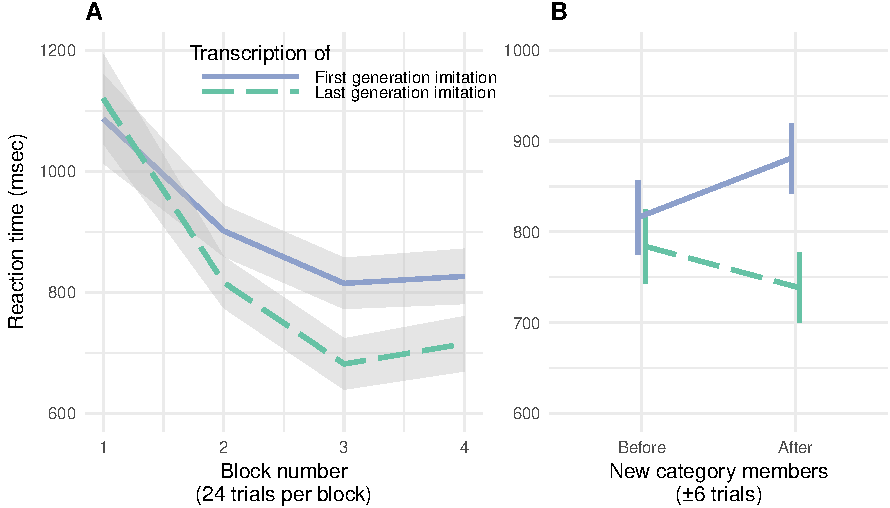
\includegraphics{fig6-1.pdf}
\caption{\label{fig:fig6}Repeated imitations made for better category
labels. Participants learned novel labels (transcriptions of first or
last generation imitations) for categories of environmental sounds. A.
Mean RTs for correct responses in the category learning experiment with
±1 SE. Participants achieved faster RTs in matching transcribed labels
to environmental sounds for labels transcribed from later compared to
earlier generation imitations. B. Cost of generalizing to new category
members with ±1 SE. After each block of trials, new environmental sounds
were introduced, requiring participants to generalize the previously
learned category labels to new category members. There was a
generalization cost for the first generation labels, but not the last
generation labels.}
\end{figure}

\subsection{Discussion}\label{discussion-2}

The results of a simple category learning experiment demonstrate a
possible benefit to the stabilization of repeated imitations on more
wordlike forms. As a consequence of being more wordlike, repeated
imitations were responded to more quickly, and generalized to new
category members more easily. These results suggest an advantage to
repeating imitations from the perspective of the language learner in
that they afford better category generalization.

\section{General Discussion}\label{general-discussion}

Imitative words are found across the spoken languages of the world
(Dingemanse et al., 2015; Imai \& Kita, 2014; Perniss et al., 2010).
Counter to past assumptions about the limitations of human vocal
imitation, people are surprisingly effective at using vocal imitation to
represent and communicate about the sounds in their environment
(Lemaitre et al., 2016) and more abstract meanings (Perlman et al.,
2015), making the hypothesis that early spoken words originated from
imitations a plausible one. We examined whether simply repeating an
imitation of an environmental sound---with no intention to create a new
word or even to communicate---produces more word-like forms.

Our results show that through simple repetition, imitative vocalizations
became more word-like both in form and function. In form, the
vocalizations gradually stabilized over generations, becoming more
similar from imitation to imitation. They also became increasingly
standardized in accordance with English orthography, as later
generations were more consistently transcribed into English words,
providing converging evidence of stabilization. In function, the
increasingly word-like forms became more effective as category labels.
In a category learning experiment, naïve participants were faster at
matching category labels derived from later-generation imitations than
those derived directly from imitations of environmental sounds. This
fits with previous research showing that the relatively arbitrary forms
that are typical of words (e.g. \enquote{dog}) makes them better suited
to function as category labels compared to direct auditory cues
(Boutonnet \& Lupyan, 2015; Edmiston \& Lupyan, 2015; e.g.~the sound of
a dog bark; Lupyan \& Thompson-Schill, 2012).

Even as the vocalizations became more word-like, they nevertheless
maintained an imitative quality. After eight generations they could no
longer be matched to the particular sound from which they originated any
more accurately than they could be matched to the general category of
environmental sound. Thus, information that distinguished an imitation
from other sound categories was more resilient to transmission decay
than exemplar information within a category. Remarkably, even after the
vocalizations were transcribed into English orthography, participants
were able to guess their original sound category from the written
\enquote{words}. In contrast to the vocalizations, participants
continued to be more accurate at matching late generation transcriptions
back to their particular source sound relative to other exemplars from
the same category.

Although the number of imitative words in contemporary languages may
appear to be very small (Crystal, 1987; Newmeyer, 1992), increasing
evidence from disparate languages shows that vocal imitation is, in
fact, a widespread source of vocabulary. Cross-linguistic surveys
indicate that onomatopoeia---imitative words used to represent
sounds---are a universal lexical category found across the world's
languages (Dingemanse, 2012). Even English, a language that has been
characterized as relatively limited in iconic vocabulary (Vigliocco,
Perniss, \& Vinson, 2014), is documented as having hundreds of clearly
imitative words including words for human and animal vocalizations as
well as various types of environmental sounds (Rhodes, 1994; Sobkowiak,
1990). Besides words that are directly imitative of sounds---the focus
of the present study --- many languages contain semantically broader
inventories of ideophones. These words comprise a grammatically and
phonologically distinct class of words that are used to express various
sensory-rich meanings, such as qualities related to manner of motion,
visual properties, textures and touch, inner feelings and cognitive
states (Dingemanse, 2012; Nuckolls, 1999; Voeltz \& Kilian-Hatz, 2001).
As with onomatopoeia, ideophones are often recognized by naïve speakers
as bearing a degree of resemblance to their meaning (Dingemanse,
Schuerman, \& Reinisch, 2016).

Our study focused on imitations of environmental sounds and more work
remains to be done to determine the extent to which vocal imitation can
ground de novo vocabulary creation in other semantic domains (Lupyan \&
Perlman, 2015; e.g., Perlman et al., 2015). What the present results
make clear is that the transition from imitation to word can be a rapid
and simple process: the mere act of iterated imitation can drive
vocalizations to become more word-like in both form and function.
Notably, just as onomatopoeia and ideophones of natural languages
maintain a resemblance to the quality they represent, the present vocal
imitations transitioned to words while retaining a resemblance to the
original sound that motivated them.

\section{References}\label{references}

\setlength{\parindent}{-0.5in} \setlength{\leftskip}{0.5in}

\hypertarget{refs}{}
\hypertarget{ref-Arbib:2012htb}{}
Arbib, M. A. (2012). \emph{How the brain got language: The mirror system
hypothesis} (Vol. 16). Oxford University Press.

\hypertarget{ref-Armstrong:2007go}{}
Armstrong, D. F., \& Wilcox, S. (2007). \emph{The gestural origin of
language}. Oxford University Press.

\hypertarget{ref-lme4:2015}{}
Bates, D., Mächler, M., Bolker, B., \& Walker, S. (2015). Fitting Linear
Mixed-Effects Models Using lme4. \emph{Journal of Statistical Software},
\emph{67}(1), 1--48.

\hypertarget{ref-Boutonnet:2015fz}{}
Boutonnet, B., \& Lupyan, G. (2015). Words Jump-Start Vision: A Label
Advantage in Object Recognition. \emph{Journal of Neuroscience},
\emph{35}(25), 9329--9335.

\hypertarget{ref-Brown:1955wy}{}
Brown, R. W., Black, A. H., \& Horowitz, A. E. (1955). Phonetic
symbolism in natural languages. \emph{Journal of Abnormal Psychology},
\emph{50}(3), 388--393.

\hypertarget{ref-Clark:1990cl}{}
Clark, H. H., \& Gerrig, R. J. (1990). Quotations as demonstrations.
\emph{Language}, \emph{66}, 764--805.

\hypertarget{ref-Corballis:2003ha}{}
Corballis, M. C. (2003). \emph{From hand to mouth: The origins of
language}. Princeton University Press.

\hypertarget{ref-Crystal:1987en}{}
Crystal, D. (1987). \emph{The Cambridge Encyclopedia of Language} (Vol.
2). Cambridge Univ Press.

\hypertarget{ref-Dingemanse:2012fc}{}
Dingemanse, M. (2012). Advances in the Cross-Linguistic Study of
Ideophones. \emph{Language and Linguistics Compass}, \emph{6}(10),
654--672.

\hypertarget{ref-Dingemanse:2014gj}{}
Dingemanse, M. (2014). Making new ideophones in Siwu: Creative depiction
in conversation. \emph{Pragmatics and Society}.

\hypertarget{ref-Dingemanse:2015cu}{}
Dingemanse, M., Blasi, D. E., Lupyan, G., Christiansen, M. H., \&
Monaghan, P. (2015). Arbitrariness, Iconicity, and Systematicity in
Language. \emph{Trends in Cognitive Sciences}, \emph{19}(10), 603--615.

\hypertarget{ref-Dingemanse:2016vd}{}
Dingemanse, M., Schuerman, W., \& Reinisch, E. (2016). What sound
symbolism can and cannot do: Testing the iconicity of ideophones from
five languages. \emph{Language}, \emph{92}.

\hypertarget{ref-Donald:2016kd}{}
Donald, M. (2016). Key cognitive preconditions for the evolution of
language. \emph{Psychonomic Bulletin \& Review}, 1--5.

\hypertarget{ref-Edmiston:2015he}{}
Edmiston, P., \& Lupyan, G. (2015). What makes words special? Words as
unmotivated cues. \emph{Cognition}, \emph{143}(C), 93--100.

\hypertarget{ref-irr:2012}{}
Gamer, M., Lemon, J., Fellows, I., \& Singh, P. (2012). \emph{irr:
Various Coefficients of Interrater Reliability and Agreement}.

\hypertarget{ref-GoldinMeadow:2016bw}{}
Goldin-Meadow, S. (2016). What the hands can tell us about language
emergence. \emph{Psychonomic Bulletin \& Review}, \emph{24}(1), 1--6.

\hypertarget{ref-PCT:1.1}{}
Hall, K. C., Allen, B., Fry, M., Mackie, S., \& McAuliffe, M. (2016).
Phonological CorpusTools. \emph{14th Conference for Laboratory
Phonology}.

\hypertarget{ref-Hewes:1973vr}{}
Hewes, G. W. (1973). Primate Communication and the Gestural Origin of
Language. \emph{Current Anthropology}, \emph{14}(1/2), 5--24.

\hypertarget{ref-Hockett:1978se}{}
Hockett, C. F. (1978). In search of Jove's brow. \emph{American Speech},
\emph{53}(4), 243--313.

\hypertarget{ref-Imai:2014dea}{}
Imai, M., \& Kita, S. (2014). The sound symbolism bootstrapping
hypothesis for language acquisition and language evolution.
\emph{Philosophical Transactions of the Royal Society B: Biological
Sciences}, \emph{369}(1651).

\hypertarget{ref-Kendon:2014eg}{}
Kendon, A. (2014). Semiotic diversity in utterance production and the
concept of 'language'. \emph{Philosophical Transactions of the Royal
Society B: Biological Sciences}, \emph{369}(1651), 20130293--20130293.

\hypertarget{ref-Klima:1980si}{}
Klima, E. S., \& Bellugi, U. (1980). \emph{The signs of language}.
Harvard University Press.

\hypertarget{ref-lmerTest:2016}{}
Kuznetsova, A., Bruun Brockhoff, P., \& Haubo Bojesen Christensen, R.
(2016). \emph{lmerTest: Tests in Linear Mixed Effects Models}.

\hypertarget{ref-Lemaitre:2014kr}{}
Lemaitre, G., \& Rocchesso, D. (2014). On the effectiveness of vocal
imitations and verbal descriptions of sounds. \emph{The Journal of the
Acoustical Society of America}, \emph{135}(2), 862--873.

\hypertarget{ref-Lemaitre:2016kz}{}
Lemaitre, G., Houix, O., Voisin, F., Misdariis, N., \& Susini, P.
(2016). Vocal Imitations of Non-Vocal Sounds. \emph{PloS One},
\emph{11}(12), e0168167--28.

\hypertarget{ref-Lewis:2009wz}{}
Lewis, J. (2009). As well as words: Congo Pygmy hunting, mimicry, and
play. In \emph{The cradle of language}. The cradle of language.

\hypertarget{ref-Lupyan:2015vic}{}
Lupyan, G., \& Perlman, M. (2015). The vocal iconicity challenge! In
\emph{The th biennial protolanguage conference}. Rome, Italy.

\hypertarget{ref-Lupyan:2012cp}{}
Lupyan, G., \& Thompson-Schill, S. L. (2012). The evocative power of
words: Activation of concepts by verbal and nonverbal means.
\emph{Journal of Experimental Psychology: General}, \emph{141}(1),
170--186.

\hypertarget{ref-Newmeyer:1992we}{}
Newmeyer, F. J. (1992). Iconicity and generative grammar.
\emph{Language}.

\hypertarget{ref-Nuckolls:1999ca}{}
Nuckolls, J. B. (1999). The case for sound symbolism. \emph{Annual
Review of Anthropology}, \emph{28}(1), 225--252.

\hypertarget{ref-Perlman:2015ip}{}
Perlman, M., Dale, R., \& Lupyan, G. (2015). Iconicity can ground the
creation of vocal symbols. \emph{Royal Society Open Science},
\emph{2}(8), 150152--16.

\hypertarget{ref-Perniss:2010fb}{}
Perniss, P., Thompson, R. L., \& Vigliocco, G. (2010). Iconicity as a
General Property of Language: Evidence from Spoken and Signed Languages.
\emph{Frontiers in Psychology}, \emph{1}.

\hypertarget{ref-Pinker:2005cv}{}
Pinker, S., \& Jackendoff, R. (2005). The faculty of language: what's
special about it? \emph{Cognition}, \emph{95}(2), 201--236.

\hypertarget{ref-Rhodes:1994au}{}
Rhodes, R. (1994). Aural images. \emph{Sound Symbolism}, 276--292.

\hypertarget{ref-Shrout:1979tg}{}
Shrout, P. E., \& Fleiss, J. L. (1979). Intraclass correlations: uses in
assessing rater reliability. \emph{Psychological Bulletin},
\emph{86}(2), 420--428.

\hypertarget{ref-Sobkowiak:1990ph}{}
Sobkowiak, W. (1990). On the phonostatistics of English onomatopoeia.
\emph{Studia Anglica Posnaniensia}, \emph{23}, 15--30.

\hypertarget{ref-Tomasello:2010or}{}
Tomasello, M. (2010). \emph{Origins of human communication}. MIT press.

\hypertarget{ref-Vigliocco:2014fc}{}
Vigliocco, G., Perniss, P., \& Vinson, D. (2014). Language as a
multimodal phenomenon: implications for language learning, processing
and evolution. \emph{Philosophical Transactions of the Royal Society B:
Biological Sciences}, \emph{369}(1651), 20130292--20130292.

\hypertarget{ref-Voeltz:2001vv}{}
Voeltz, F. E., \& Kilian-Hatz, C. (2001). \emph{Ideophones} (Vol. 44).
John Benjamins Publishing.


\clearpage
\renewcommand{\listtablename}{Table captions}
\listoftables

\clearpage
\renewcommand{\listfigurename}{Figure captions}
\listoffigures



\end{document}
